\documentclass[11pt,a4paper]{article}
% Locale and font
\usepackage[utf8]{inputenc}
\usepackage[T1]{fontenc}
\usepackage[english]{babel} % Set language here

% Layout
\usepackage{hyperref}
\usepackage{float}
\usepackage[margin=1cm]{caption} % Additional margin for captions
\usepackage{geometry}
\geometry{margin=1.25in} % Margin for dokument (default in Word is 1.25 inches)

\setlength{\parskip}{1em} % Skip for paragraphs
\setlength{\parindent}{0em} % Indentation for paragraphs

\usepackage[dvipsnames]{xcolor} % Color

% #########################
% Citations
\bibliographystyle{unsrt} % Set reference system here

% #########################
% Math
\usepackage{amsmath}
\usepackage{amssymb}
\usepackage{mathtools}
\usepackage{textgreek}
\usepackage{mathrsfs}

% #########################
% Physics/Chemistry
%   Chemical and nuclear reactions
%\usepackage[version=4]{mhchem} 

% Tables and plots
%   Figures
\usepackage{tikz}
\usepackage{svg}
\usepackage{graphicx}
\usepackage{subcaption}

%   Nicer tables
\usepackage{booktabs}

% #########################
% Text information
\newcommand{\Foursename}{Astrophysics 1} % Set course name here
\newcommand{\Fassignment}{Bonus Exercise} % Set assignment title here
\newcommand{\Foursecode}{\texttt{1FA204}} % Set course code here
\newcommand{\Fauthor}{Oliver Kraft} % Set author here
\newcommand{\Femail}{oliver.kraft.9720@student.uu.se} % Set email here
\newcommand{\Fersonalnumber}{20010609-XXXX}
\date{December 2021} % Set date here

%   Parameters for use in text
\title{\Foursename\, -\, \Fassignment}
\author{\Fauthor}

% #########################
% Header and footer
\usepackage{fancyhdr}

\lhead{\Foursecode}
\chead{\href{mailto:\Femail}{\texttt{\textcolor{lightgray}{\Femail}}}}
\rhead{\texttt{\Fauthor}}
\setlength{\headheight}{15pt}

\rfoot{\texttt{Page \thepage}} % Page text can be adjusted here
\lfoot{}
\cfoot{}

\fancypagestyle{plain}{
    \fancyfoot{} % Remove footer
}

\pagestyle{fancy}

% #########################
% Miscelaneous
\usepackage{pdfpages} % Include a whole pdf with \includepdf[pages=-]{file.pdf}



% Code test:
\usepackage{minted}

\begin{document}

    \begin{titlepage}
    \centering
    
\includegraphics[width=12cm]{logos/UU_logo.eps}
    \vfill
    {\bfseries\Large
    \makeatletter
    \@title\\
    \@date\\
    \vskip1cm
    \@author\\
    \vskip0.5cm
    \makeatletter
    }
    \vfill
    \vfill
\end{titlepage}
    \clearpage
    \section*{\Fassignment}

    \textbf{Note:} I'm using the following notation for labeling the plots: \texttt{[age]y[metallicity]m}.
    For instance the isochrone with stars aged $4.69 \cdot 10^9$ years with metallicity $0.0152$ would be denoted as: \texttt{4.69e9y0.0152m}.

    \begin{figure}[h]
        \centering
        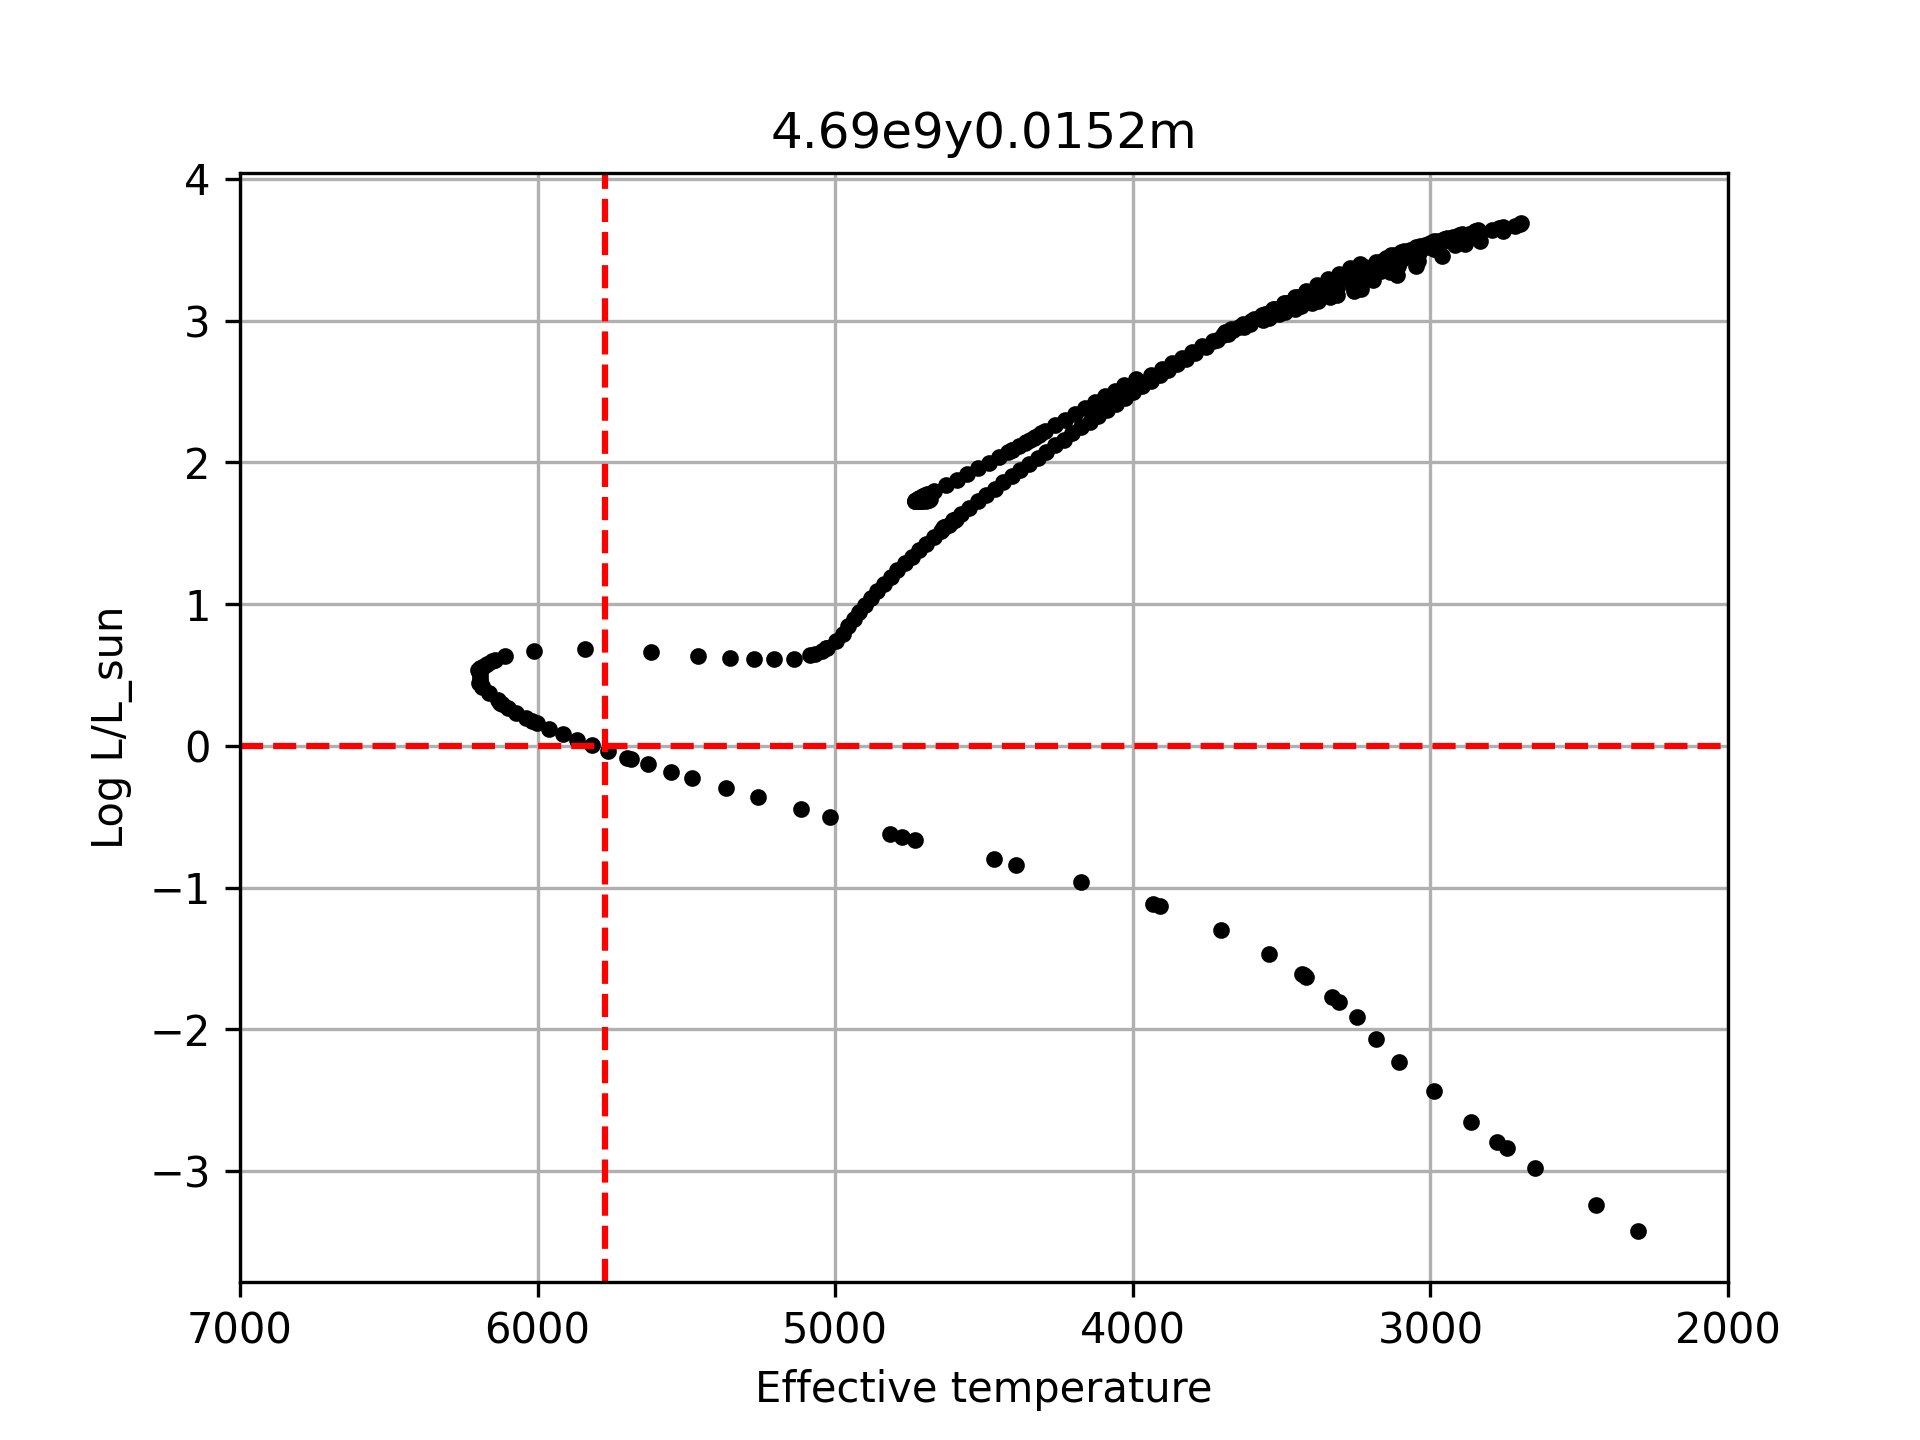
\includegraphics[width=12cm]{figures/4.69e9y0.0152m}
        \caption{HR plot of cluster with age $4.69 \cdot 10^{9}$ years and metallicity 0.0152.}
        \label{fig:ogHR}
    \end{figure}

    \textbf{1)} \textit{At which stellar initial mass, effective temperature and stellar luminosity is the turnoff point? What does this point reflect, physically?}

    Stellar initial mass: 1.69\\
    Effective temperature: approx 6200 K\\
    Luminosity: $\textrm{LogL} = 0.5 \Rightarrow L/L_sun = 3.16 \Rightarrow L = 1.216 \cdot 10^{27} \textrm{ W/m}^2$
    
    \textbf{2)} \textit{At which stellar initial mass, effective temperature, and stellar luminosity is the base of the Red Giant Branch?}

    Stellar initial mass: 2.45 \\
    Effective temperature: approx 6100 K ($\textrm{logTe} \approx 3.71$) \\
    Luminosity: $\textrm{LogL} = 0.575 \Rightarrow L/L_{sun} = 3.758 \Rightarrow L = 1.4461 \cdot 10^{27} \textrm{ W/m}^2$
    
    \textbf{3)} \textit{How has the appearance of the main sequence changed, compared to that shown in Fig. 1?
    What is the reason for this, in terms of nuclear fuel?}

    More stars have deviated from the main sequence, the turnoff point has moved lower in temperature.
    The reason for this is that as the cluster aged more stars have had time to expend their fuel and turned onto the red giant branch.
    As the stars transition from burning hydrogen to helium the outward pressure increases causing the star to expand and the temperature to drop.
    This causes the stars to appear redder.

    \textbf{4)} \textit{How old will the Sun be when it leaves the main sequence?
    Please estimate this by making a few more plots, varying the age of the cluster.}

    \begin{figure}
        \centering
        \includegraphics[width=]{}
    \end{figure}

\end{document}
